\documentclass[11pt]{article}
\usepackage{graphicx}
\usepackage{amsmath}
\usepackage{booktabs}
\usepackage{geometry}
\usepackage{hyperref}
\usepackage{float}
\usepackage{setspace}
\geometry{margin=1in}
\setlength{\parindent}{0pt}

\begin{document}

\begin{center}
    \vspace*{0.5cm}
    {\Huge\bfseries Earnings Case Study\par}
    \vspace{0.8cm}
    {\large Nathan Brown\par}
    {\large \today\par}
    \vspace{1cm}
\end{center}

\tableofcontents
\newpage

\section{Duolingo: DUOL}
    \subsection{2023-02-28 Earnings Report}
        \begin{itemize}
            \item \textit{Earnings Summary:} DUOL reported sixth consecutive quarter of user/growth acceleration with DAUs +62\% YoY to 16.3M and MAUs +43\% to 60.7M. Other key KPIs (total revenues, adjusted EBITDA, paid subscriber count) all increased by 40\%+, soothing worries about profitability saturation.
            \item \textit{Price Action:} Sideways price action following uptick in growth from early 2023. Earnings report led to heavy 22\% spike (on next trading day) with heavy (4x) volume followed by consistent gains over the next several weeks. DUOL also announced two weeks later (on Mar 14) that ``Duolingo Max'' would be powered by GPT-4. This captured AI hype and led to a further up-and-to-the-right movement.
            \begin{figure}[h]
                \centering
                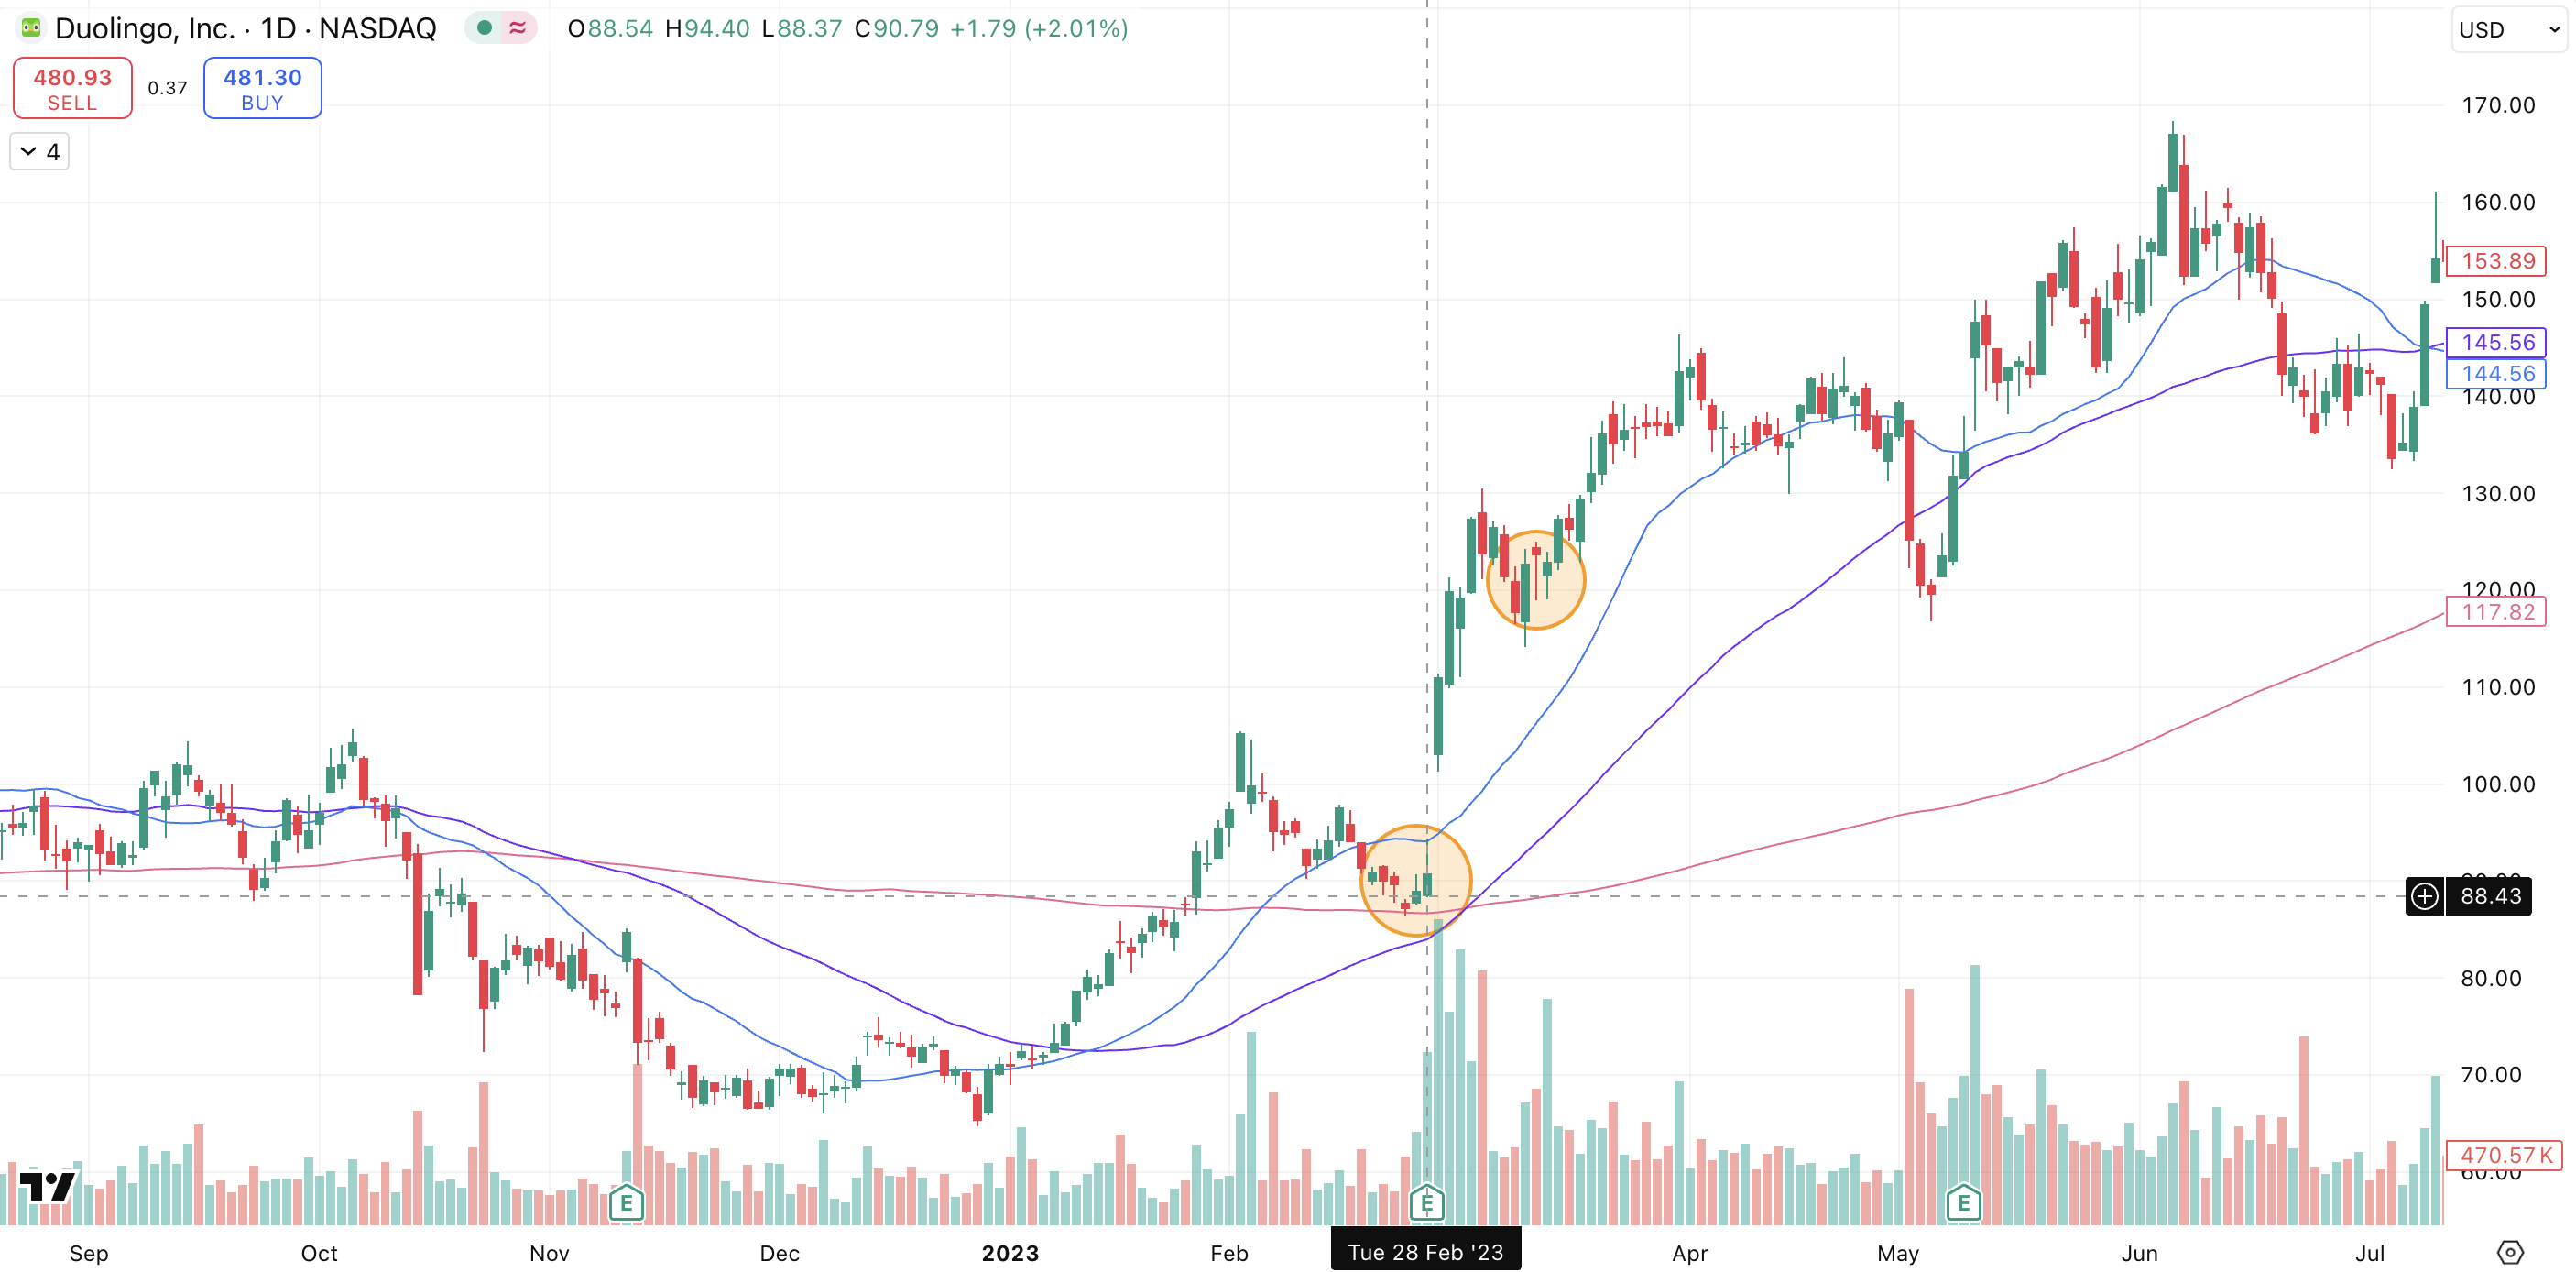
\includegraphics[width=0.8\linewidth]{images/DUOL1.png}
                \caption{1st circle indicates earnings report, 2nd circle indicates AI announcement}
            \end{figure}
        \end{itemize}
    \subsection{2025-05-01 Earnings Report}
        \begin{itemize}
            \item \textit{Earnings Summary:} Duolingo posted another strong quarter, with GAAP EPS of \$0.72 beating consensus by 20¢ and revenue climbing to \$231M (+4\% vs. Street). It marked the company’s first-ever 10M+ paid subscriber quarter (10.3M, +40\% Y/Y), as the freemium-to-paid funnel remained robust. User growth reaccelerated once again — DAUs rose 49\% Y/Y to 46.6M, and the DAU/MAU ratio improved to 35.8\%, pointing to higher engagement and retention. Adj. EBITDA margin expanded 900 bps Y/Y to 27\%, with free cash flow margin at 24\%. Management also raised full-year revenue guidance and signaled continued operating leverage, easing concerns about cost pressures tied to AI investments.
            \item \textit{Price Action:} Shares spiked over 20\% on high volume following the print. The rally came on elevated volume and was supported by a flurry of analyst upgrades and bullish headlines calling Duolingo a “consumer-AI showcase.” Investors appeared especially encouraged by traction in Duolingo Max, ongoing AI content scaling, and strong user/subscriber trends despite tough comps. The stock continued drifting upward in the days that followed, fueled by optimism around new product verticals and gross margin expansion potential.
            \begin{figure}[h]
                \centering 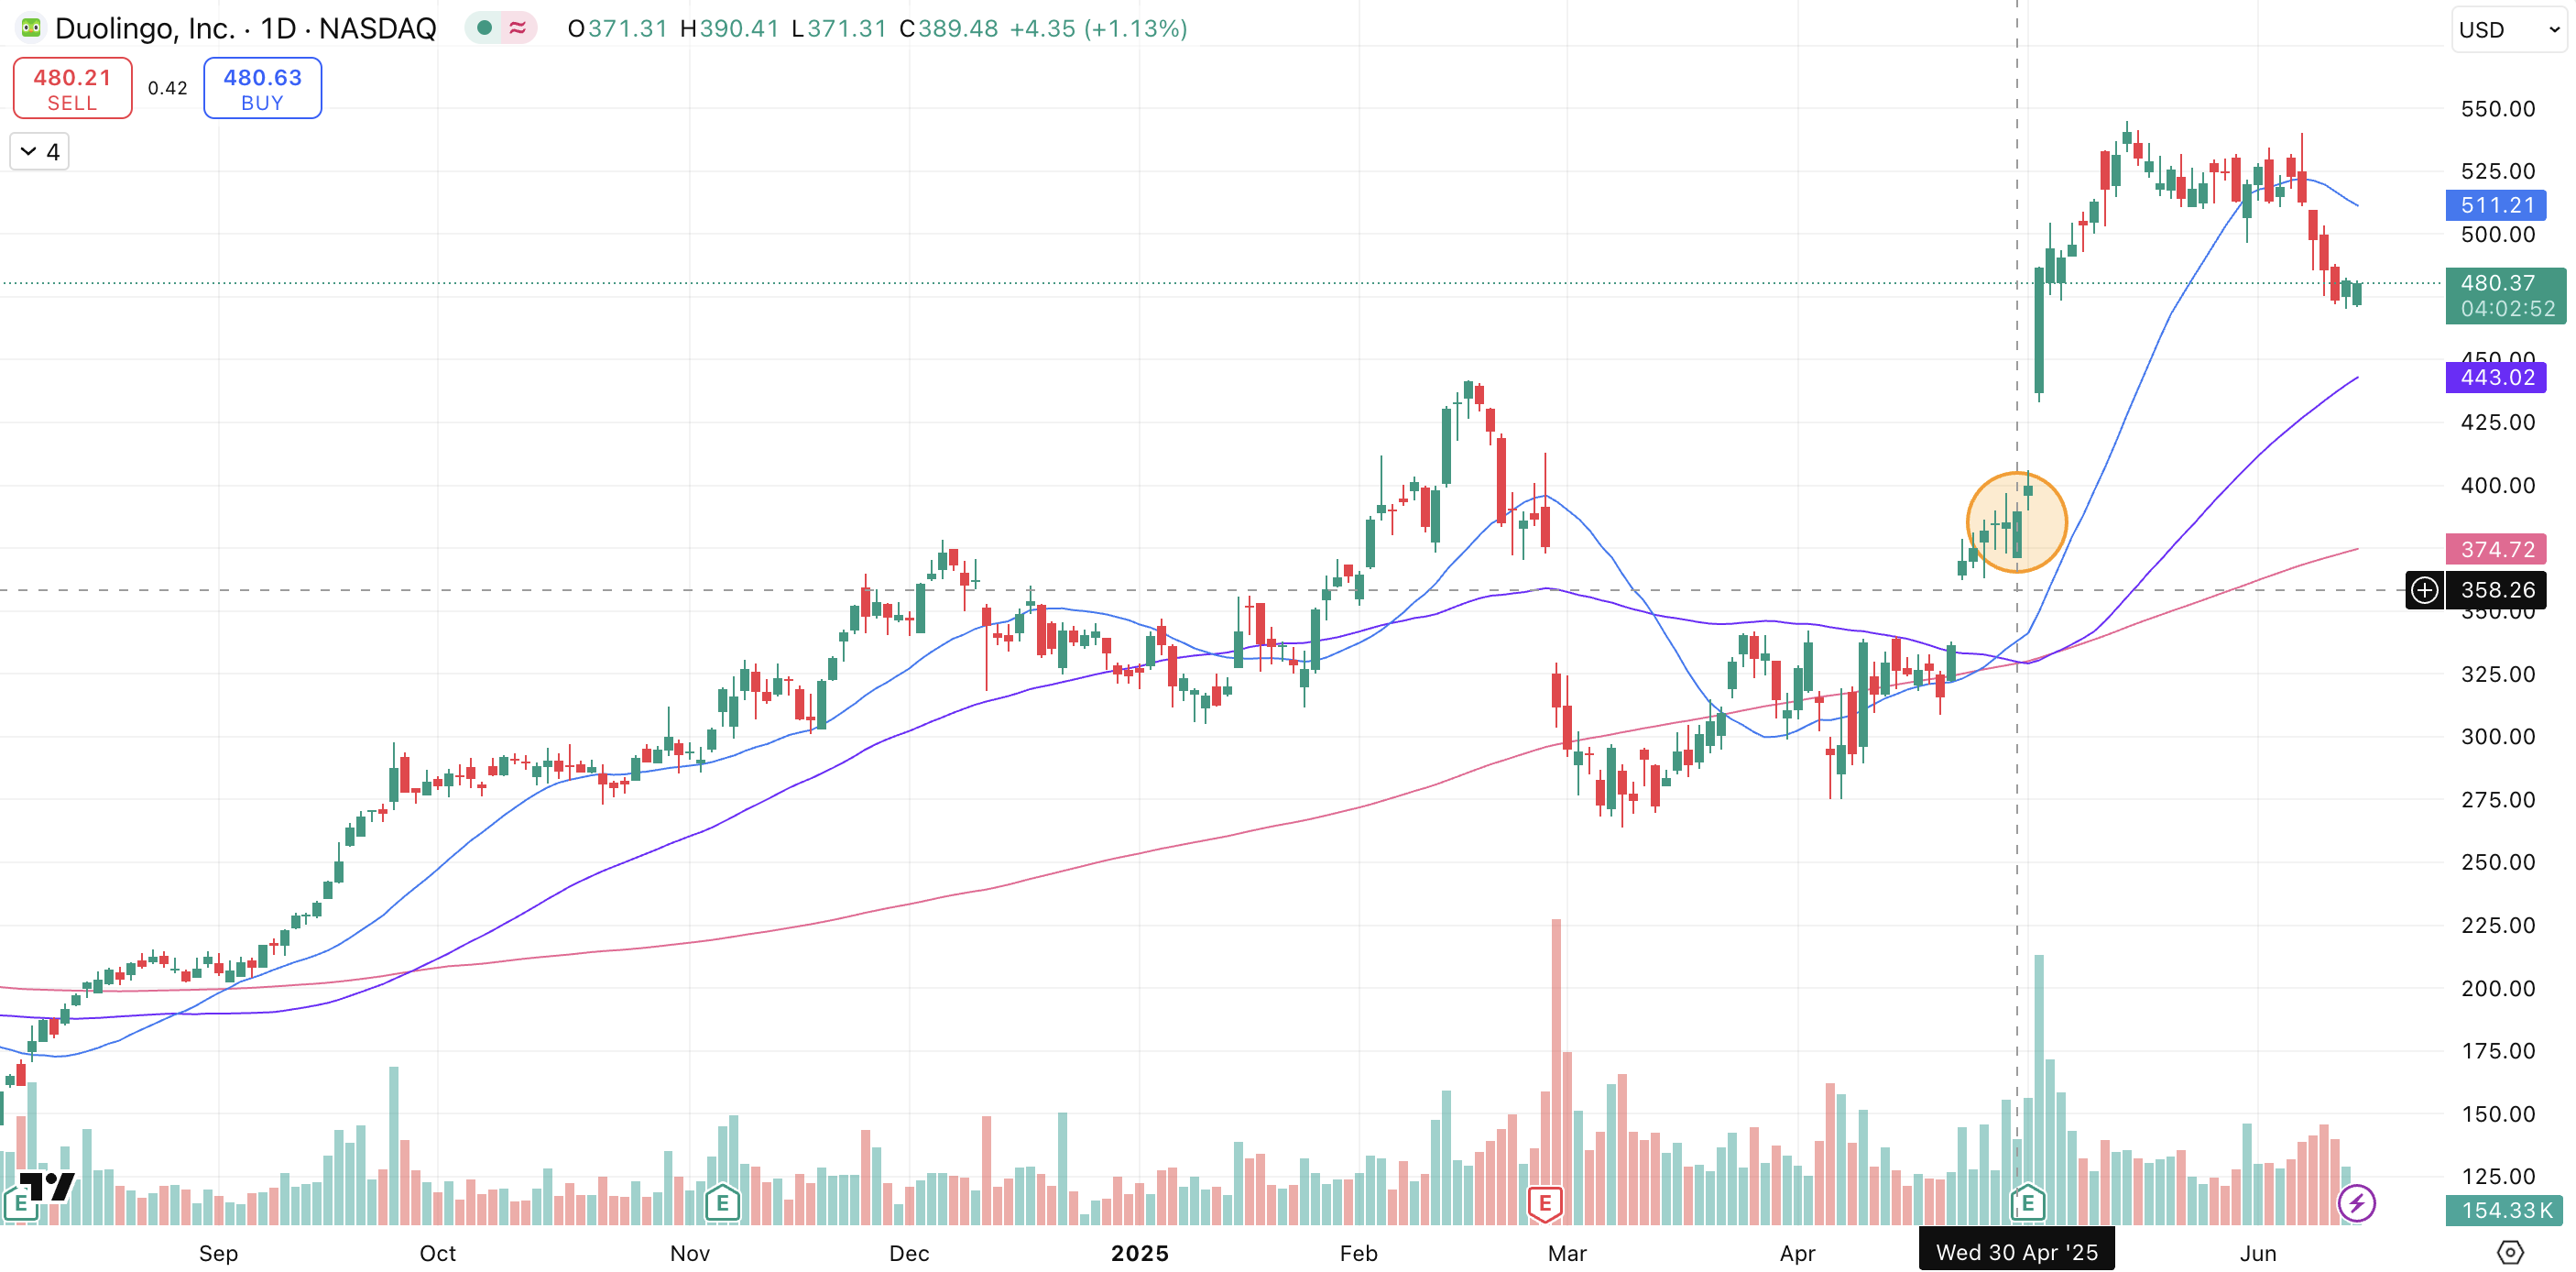
\includegraphics[width=0.8\linewidth]{images/DUOL2.png}
                \caption{Stock surged post-earnings on stronger-than-expected results and bullish guidance.}
            \end{figure}
        \end{itemize}
    \subsection{Pattern}
        The stock rallied on a rare combination of strong, consistent user and subscriber growth, expanding margins, and clear progress in AI integration—notably with Duolingo Max and AI-driven content creation—which reinforced confidence in both near-term execution and long-term scalability.
\section{LUNR}
    \subsection{2024-02-15 Moon Mission}
\end{document}
